\begin{definition} 
    \label{def:graph}
    Let \(\Sigma\) be a finite set of labels. A \textbf{directed edge-labeled multigraph} is an ordered pair \((G,\lambda)\) where \( G \) is an unlabeled graph and \( \lambda : E(G) \rightarrow \Sigma\) is an edge-labeling function. 
    It is called \textbf{finite} if its underlying unlabeled graph is finite.
    Throughout, a directed edge-labeled multigraph will be simply referred to as a \enquote{labeled graph} when the context makes it clear.
     By $a : s\overset{l}{\rightarrow} t$, we denote the arrow $a$ labeled by $l$ from $s$ to $t$.
\end{definition}
 The definition of labeled graphs extends the definition of unlabeled graphs, as unlabeled graphs can be seen as labeled graphs with a single label for all edges, i.e., the label function is a constant function.

  A homomorphism of labeled graphs is a homomorphism of unlabeled graphs that preserves the labels assigned to the edges. 
\begin{example}
    Edges of a labeled graph are directed and labeled by elements of a finite set of labels. Between any two nodes, there can be multiple edges, and loops are allowed. An example of a labeled graph is shown in~\autoref{fig:preliminaries:labeled_graph}.
    \begin{figure}[!ht]
       \centering
        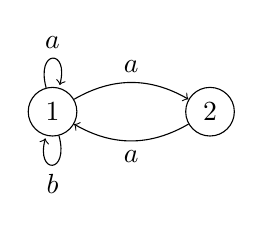
\begin{tikzpicture}
            \graphbox{}{0mm}{0mm}{32mm}{28mm}{-10mm}{-14mm}{
                \node[draw,circle] (1) at (0,0) {1};
                \node[draw,circle] (2) at (2,0) {2};
                \draw[->] (1) edge[loop above] node[midway, above] {$a$} (1) ;
                \draw[->] (1) edge[loop below] node[midway, below] {$b$} (1) ;
                \draw[->] (1) edge[bend left] node[midway, above] {$a$}  (2)  ;
                \draw[->] (2) edge[bend left] node[midway, below] {$a$} (1)   ;
            }
        \end{tikzpicture}
        \caption{Labeled graph}
        \label{fig:preliminaries:labeled_graph}
    \end{figure}

\end{example}